\section{Background and Motivation}
{
    \label{background}

    Artificial Intelligence (AI) is one of the fastest growing technology domains, involving academic research, businesses, and users. The enormous investment in AI led to groundbreaking applications in a diverse set of areas. AI is used for accelerating the discovery of drugs (e.g., \cite{Stark2022}, \cite{Ross2022}), driving efficiencies at work (e.g.,~\cite{Puri2021}), discovering new materials towards renewable storage (e.g.,~\cite{Zitnick2020}), and more. At the same time, we are also in the midst of a heated debate about the potential of AI to harm (e.g., \cite{AIdanger}). Risks frequently associated with AI include, fake news, biases, job losses, and, the enormous environmental cost. 

    The amount of compute used to train deep learning models have increased $300,\!000 \times$ in six years~\cite{Schwartz2019}. Data has increased significantly, reaching exabyte scale~\cite{Wu2022}. The data size increase has led to a super-linear growth trend in model size~\cite{Wu2022}. For example, GPT3 based language translation tasks have increased in size $1000 \times$ (\cite{Brown2020}). In contrast, systems' memory capacity only grew moderately, which has motivated a variety of scale-out infrastructure solutions (e.g.,~\cite{Patterson2021,Wu2022}), involving thousands of AI accelerators and other specialized systems. There is no doubt that these trends come with a dire environmental cost (stemming both from embodied and operational costs). Indeed, multiple researchers and practitioners have raised the alarm on the environmental cost of AI, and offered a calls-to-action (\cite{Strubell2019,Lacoste2019,Henderson2020,Schwartz2019}). 

    Meanwhile, a recent development in the field of AI is foundation models (FMs) coming to the front stage (e.g., ~\cite{Rishi2022}). FMs are trained on very broad datasets using self supervision at scale. One of the interesting characteristics of foundation models is that through transfer learning~\cite{Thrun1998} they can be adapted (e.g., fine-tuned, or distilled) to a wide range of downstream tasks. In fact, the majority of state-of- the-art NLP models are now adapted from one of a few foundation models, such as BERT~\cite{Devlin2018}, RoBERTa ~\cite{Liu2019}, BART~\cite{Lewis2019}, T5~\cite{Raffel2020}, BLOOM~\cite{Workshop2023Bloom}, LLaMA ~\cite{Touvron2023}. Foundation models are not new, but the scale, scope, and emergent capabilities of foundation models in the last few years have exceeded everyone's imagination. For example, GPT-3 has $175$ billion parameters (in comparison with the `modest' $1.5$ billion parameters of GPT-2), and it can be adapted via natural language prompts to perform a range of tasks despite not being trained explicitly to do many of those tasks~\cite{Brown2020}. Proponents of foundation models claim that the enormous amount of upfront carbon cost to train a broad model is balanced in the `big picture' by the low cost of re-using it via fine-tuning or distillation for a particular task (e.g., \cite{Rishi2022}). Alas, with no unified metric that analyses the entire provenance chain of models, datasets, and their associated cost, it is very hard to substantiate or refute this claim. 

    In this position paper, we apply broad knowledge of sustainability principles, protocols and standards, including the GHG Protocol (\cite{GHG-Protocol}), and the accompanying guidance document for cloud services (\cite{GHG-Guidance}, chapter~$4$), and product Life Cycle Assessment principles (LCA)~\cite{LCA}, to the domain of AI, in order to develop metric that can be meaningfully used to drive sustainability mindset and examine trade-offs across the life cycle of AI models, and across the `supply-chain' of models and datasets (see Fig.~\ref{fig:model_supply_chain}). As in~\cite{Gandhi2022}, and also as in the Software Carbon Intensity (CSI) specification offered by the Green Software Foundation~\cite{GSF}, we focus on a unit of work submitted on behalf of an end-user, i.e., inference jobs in the case of AI, as the primary object of interest. The metric is meant to capture the actual amortized sustainability cost of a job, taking into account operational overheads and associated embodied cost. 

    \begin{figure}[!t]
        \centering
        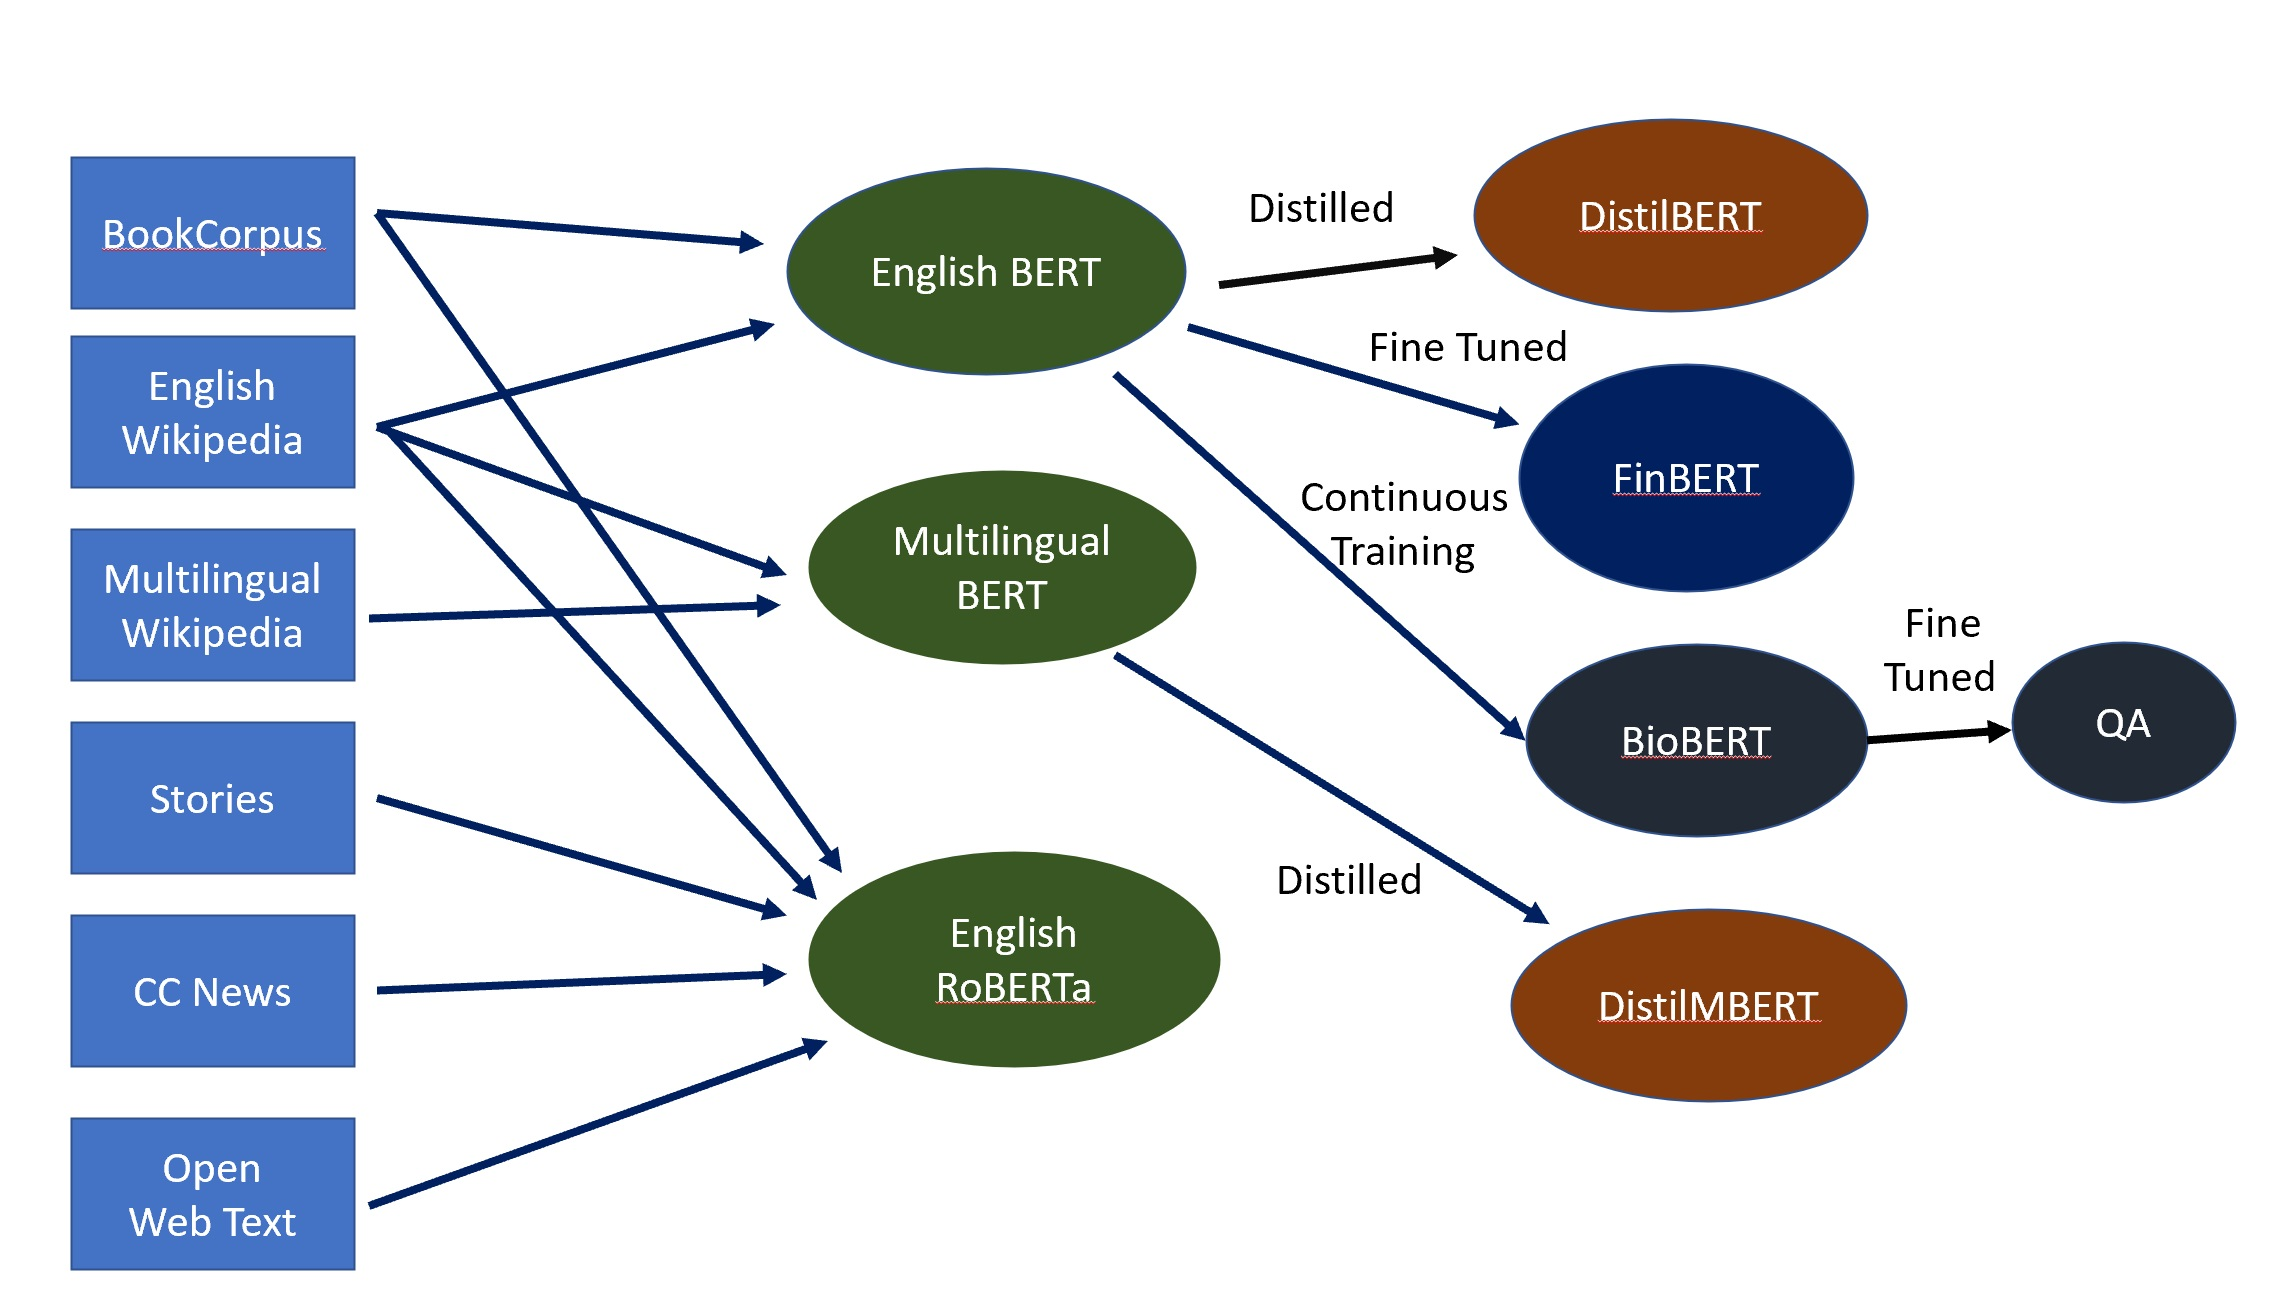
\includegraphics[width = \linewidth]{Figures/sustain1.jpg}
        \caption{The `Supply Chain' of datasets and models}
        \label{fig:model_supply_chain}
    \end{figure} 
    
    We leverage and expand the metrics defined in~\cite{Gandhi2022}, concerning the sustainability cost of jobs. Specifically, we define and motivate a new term \textit{Embodied Product Cost} for the sustainability cost of software, such as the development and testing of platforms delivered as an always running service (such as AWS's Lambda~\cite{Lambda}), and, in the domain of AI, the preparing of datasets, and training of models. We then expand the definition of job sustainability cost metrics ($JSC$ and $ASC$), to also factor in the associated embodied product cost. The expanded definition can contribute towards accuracy and completeness of job sustainability metrics. We then show how to apply this expanded definition to the area of AI. To summarize, the contribution of our paper is as follows:
    
    \begin{enumerate}
        \item We define a new metric \textit{Embodied Product Cost}, that aims at expressing the `embodied' carbon of software assets, i.e., the carbon cost of `manufacturing' a software asset, such as the development and testing of an on-line platform, or the pre-deployment training of an AI model.
        \item We expand the definitions of Job Sustainability Cost ($JSC$), and Amortized Sustainability cost ($ASC$), defined in~\cite{Gandhi2022} to factor-in the operational cost of the software asset used as the context of the execution of the job, as well as, the `embodied' costs of these software assets. The expanded definitions can be used generally for any data center job, not just AI, and contribute towards accuracy and completeness.
        \item We specialize and apply these new metrics to the case of AI. We show how our approach can promote a sustainability mind-set, and in particular can be used to analytically prove or refute the claim that foundations model re-use for downstream tasks is advantageous to the environment, relative to the construction of smaller more specific models, from scratch.
        \item We analyse the new opportunities for sustainability based research across the life-cycle and provenance chain of models.
    \end{enumerate}

    \subsection{Related Work}
    {
        Sustainable computing has gained significant attention since a decade ago, owing to the escalating demand for computing power in Cloud computing and hyper-scale data centers, which has resulted in a significant surge in energy consumption at the data center and energy proportional computing~\cite{Barroso2013}. To address this concern, there have been continuous efforts aimed at reducing power/energy consumption across different levels, ranging from chip/HW components~\cite{Jouppi2023,Jiang2020,Capra2020} to data center scale~\cite{Lee2017,Xia2017,Dayarathna2016,Kanagasubaraja2022}, including cooling techniques (Power Usage Effectiveness, PUE) and/or total cost ownership (TCO)~\cite{Zhang2021,Mukherjee2020,Chauhan2019,Rostirolla2022}.

        Multiple recent works take a holistic view of the problem area of sustainability in computing. {Gupta et al.}~\cite{Gupta2020} posits that attention must be given to the embodied emission of systems, which is becoming the dominant factor in the carbon cost of computing environments. \cite{Chien2020} argues that we need to replace static metric such as PUE and grid emission factors (CI) with dynamic, time series based, metric to enable de-carbonization of data centers by co-optimization. We agree with these assertions and believe they are complementary to the approach presented here. The most relevant to this paper is the work by {Gandhi et al.}~\cite{Gandhi2022} that argues that we should focus on the unit of work performed (namely, \textit{a job}), and, include in its amortized sustainability cost also a `slice' of the embodied emission cost of the systems used for the execution and other operational overheads such as for cooling. This approach agrees with the software Carbon Intensity (SCI) specification~\cite{SCI}, put forward by the Green Software Foundations~\cite{GSF}. We agree that we should aim at amortizing all these aspects into the carbon sustainability cost of jobs. Toward that goal, we posit that we are neglecting to consider additional aspects associated with the \textit{software product(s)} used as an execution context for the job. Examples of software products are a software platform, deployed as an always-running service, required for the execution of jobs (such as a serverless job running on the AWS Lambda platform service~\cite{Lambda}), and, in the domain of AI, a model, that is used to serve inference requests initiated by end users. In both these cases there is a significant overhead associated with (1) the on-going maintenance of the product such as service operations, or, model continuous re-training, and, (2) the up-front construction of the product (including, development and testing, or, data preparation and training). We propose new metrics, that build on the previous ones, but include these two neglected factors.

        In the area of AI, an astounding amount of progress has been accomplished on the systems side, to design energy efficient accelerators specifically for AI workloads, optimized for metrics multiplication, and incorporating low precision, and low voltage (e.g., \cite{Agrawal2016,Brooks2000}). Beyond the lens of system design, data scientists spend most of their attention fiercely competing over accuracy as a primary goal, and time-to-value as a secondary goals (e.g., ~\cite{Liu2019}). The papers ~\cite{Strubell2019} and ~\cite{Schwartz2019}, were among the first to call attention to the issue of the environmental cost of AI, focusing in particularly, on the training phase of the life cycle. {Michel et al.}~\cite{Lenherr2021}, offers a single metric that can be used to compare the energy efficiency of different models with respect to their complexity (e.g., based on number of classes), and their accuracy. The work~\cite{Patterson2021}, asserts the difficulty in assessing the $gC0_{2e}$ of AI models, which necessitate considering the energy mix in the location of the training, and the hardware architecture used. By considering these two aspect, they correct previous estimates, such as in~\cite{Strubell2019} by as much as $88 \times$. They also join the call to define standards and norms for Sustainable AI. Lastly, {Wu et al.}~\cite{Wu2022}, is first to suggest we need a \textit{holistic} approach to Sustainable AI that considers \textit{all stages of the life cycle}, and also including the embodied emission of systems used. Some of the interesting findings in this paper are: (1) that the often completely overlooked data preparation phase, consumes in some cases an equal amount of energy as the training phase, and, (2) that the ratio between energy spent in different phases of the model life cycle  \textit{varies across different use cases}. These two key observations contributed to motivating this position paper. First, we focus on two specific software assets: datasets, and models. By defining the concept of `embodied emission of software' we capture the gCO2e cost of pre-preparation of data set, and pre-training of models. Further we factor-in these costs, as well as the, mostly overlooked, cost of maintaining a model with frequent re-training, in amortizing the gCO2e cost per inference transaction, which is the unit of work performed on behalf on an end user. We postulate that this  approach will allow us to analytically compare different strategies, e.g., the size of the model used, and whether it was distilled based on a previous model, or trained from scratch. 
    }

    %\begin{figure*}[tb]
    %    \centering
	%    \begin{minipage}{.45\columnwidth}
	%	    \centering
    %        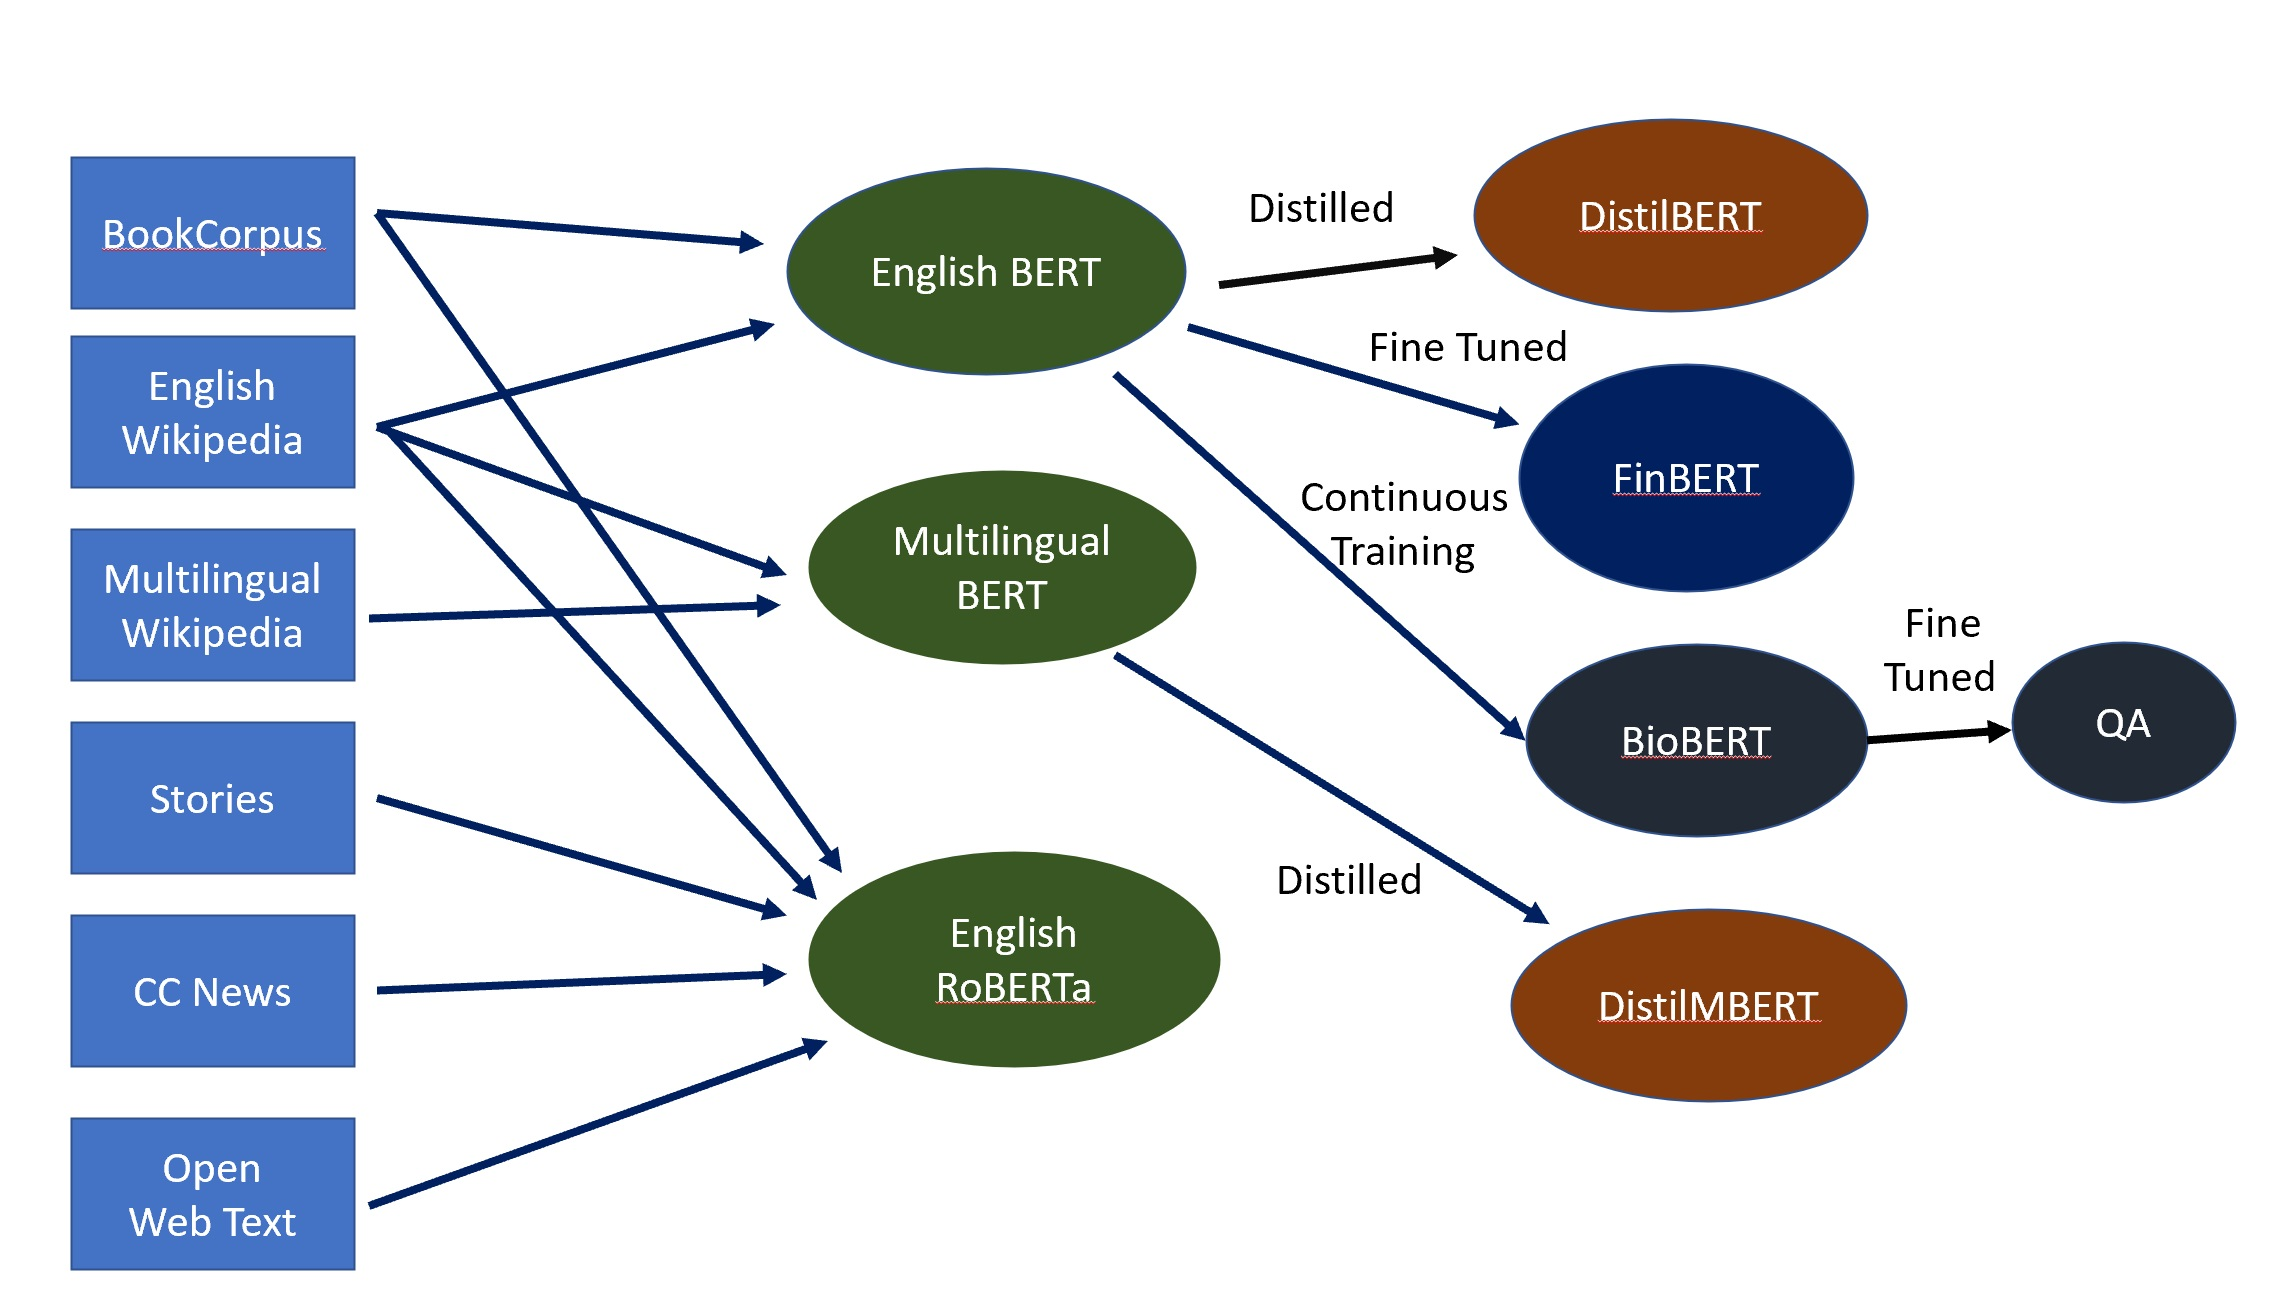
\includegraphics[width=\textwidth]{Figures/sustain1.jpg}
    %        \caption{The `Supply Chain' of datasets and models.}
    %        \label{fig:model_supply_chain}
    %    \end{minipage}
	%    \begin{minipage}{.45\columnwidth}
	%	    \centering
    %        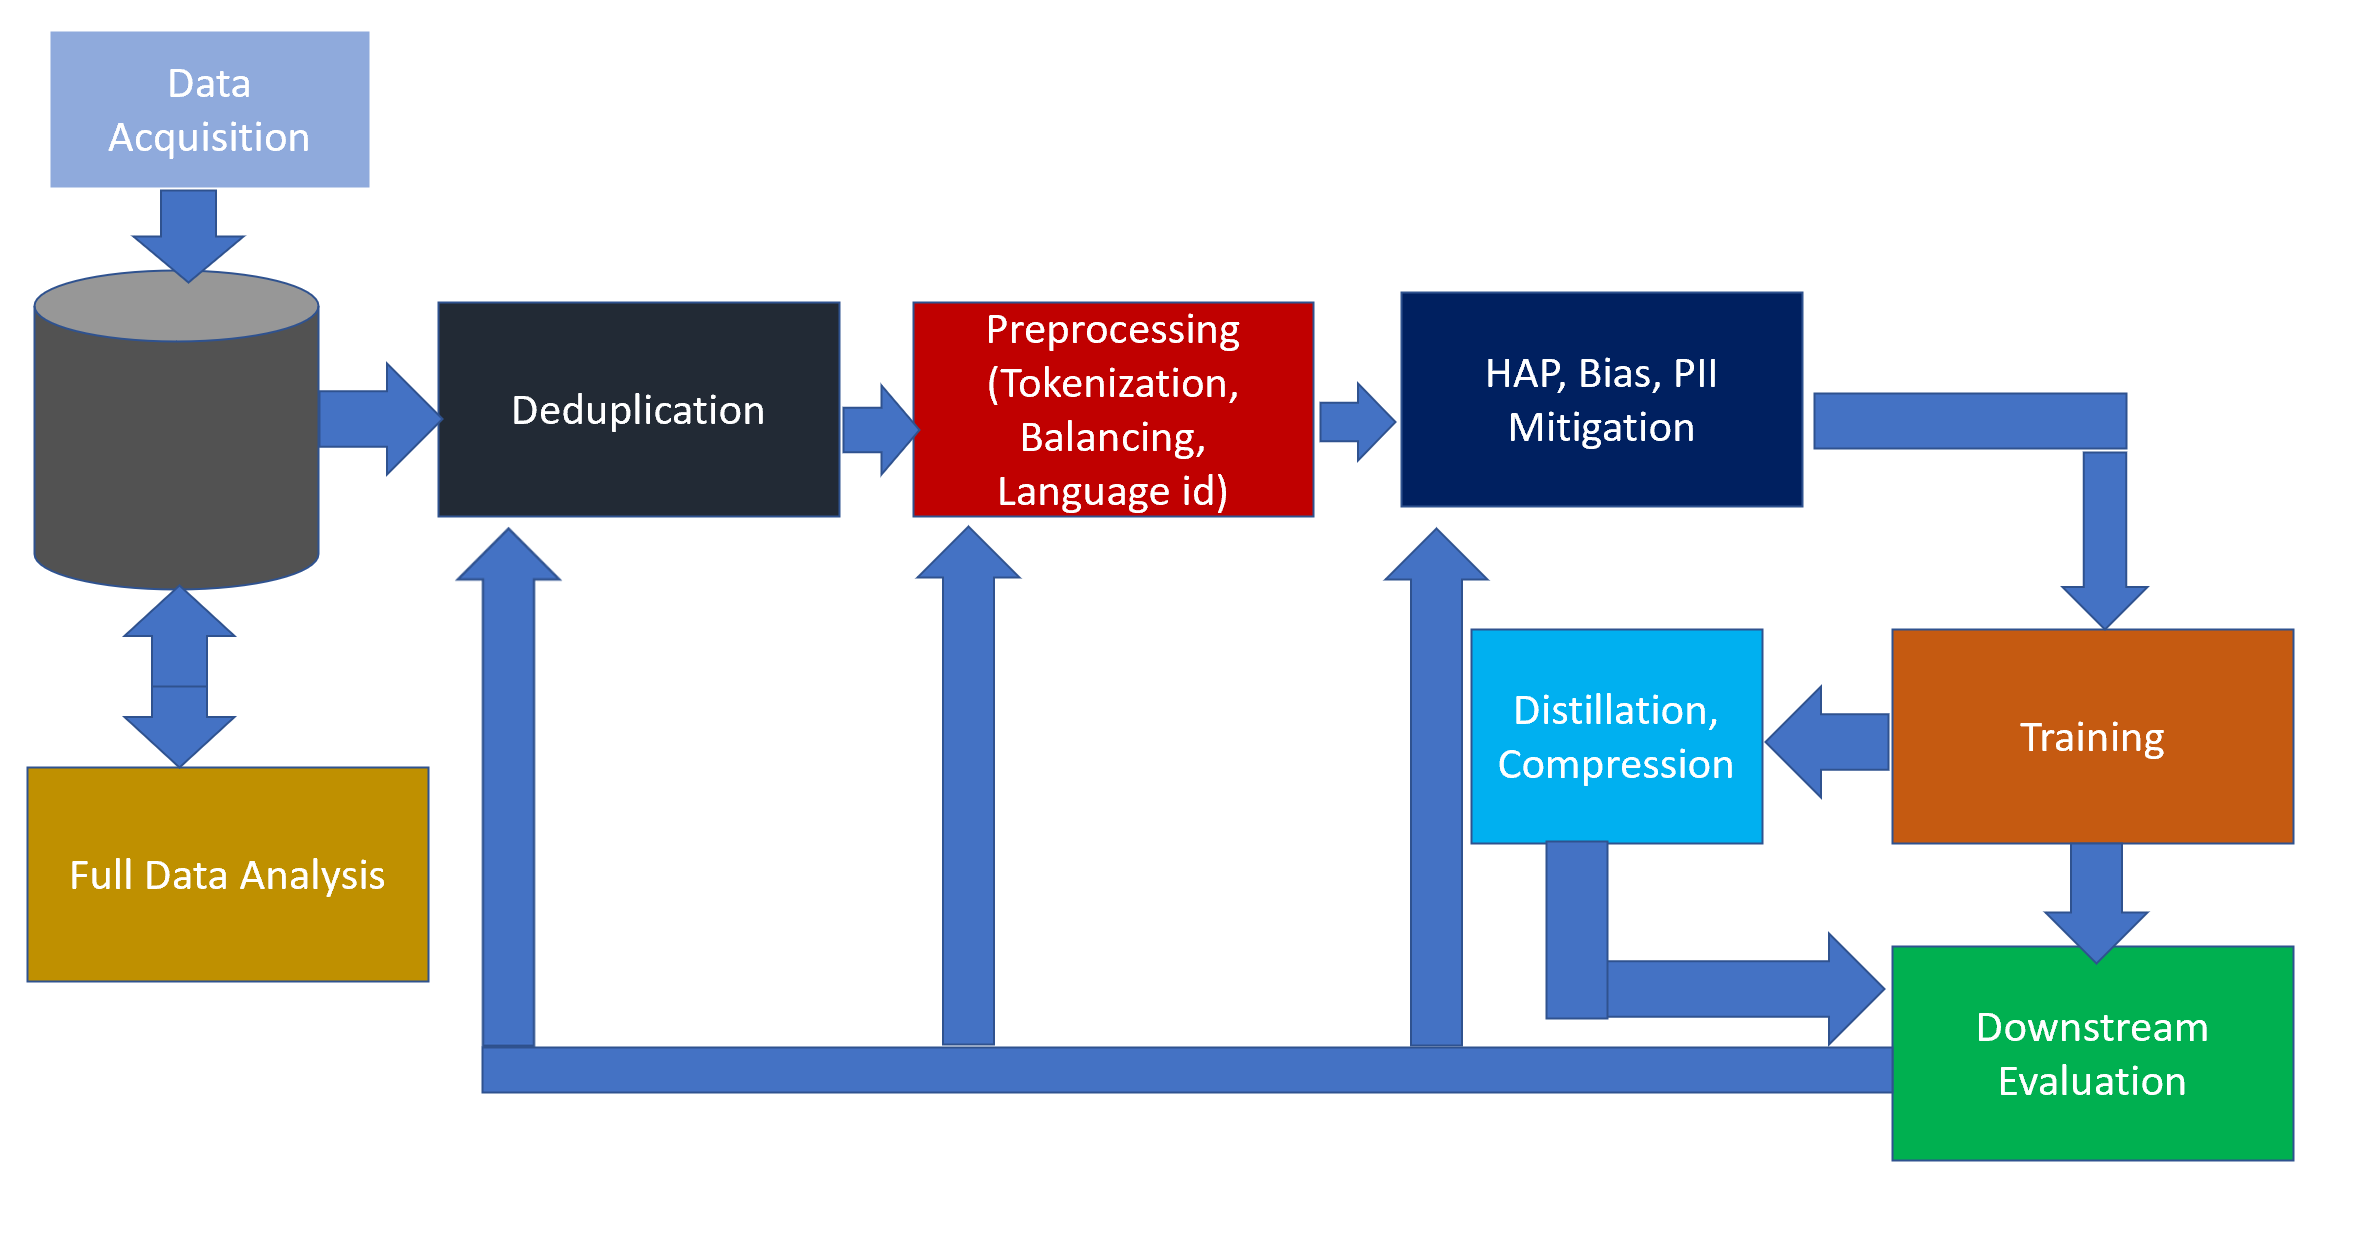
\includegraphics[width=\textwidth]{Figures/sustain3.png}
    %        \caption{A typical preprocessing pipeline.}
    %        \label{fig:model-preprocess}
    %    \end{minipage}
    %\end{figure*}
    
    \subsection{The life cycle of an AI model}
    {
        \label{life-cycle}

        To fully understand the real environmental impact, and to be able to develop the right approach to assess the impact, we must closely examine the model life cycle, end-to-end, including: data collection, model exploration and experimentation, model training, model distillation, and fine tuning, deployment, and then re-training, and inference cost. 

        A pre-processing pipeline, needed to curate data for training a model, could consist of the following steps: Data acquisition: via crawling (for NLP), or running simulations (materials or physics); De-duplicating:  to ensure there is one copy of a document from multiple sources; Selecting documents of certain languages of interest; Splitting the documents into sentences for training; Identifying Hate Abuse Profanity and PII information one may want to filter; Forming the data files for training based on a given format. For example, NLP datasets such as  Wikipedia,  Stories,  OpenWebText, BookCorpus, CC News are constructed via web crawling. Each of them could potentially be processed through all the above steps before it is ready for being used for training. Fig.~\ref{fig:model-preprocess} shows such a pipeline. 

         \begin{figure}[!t]
             \centering
             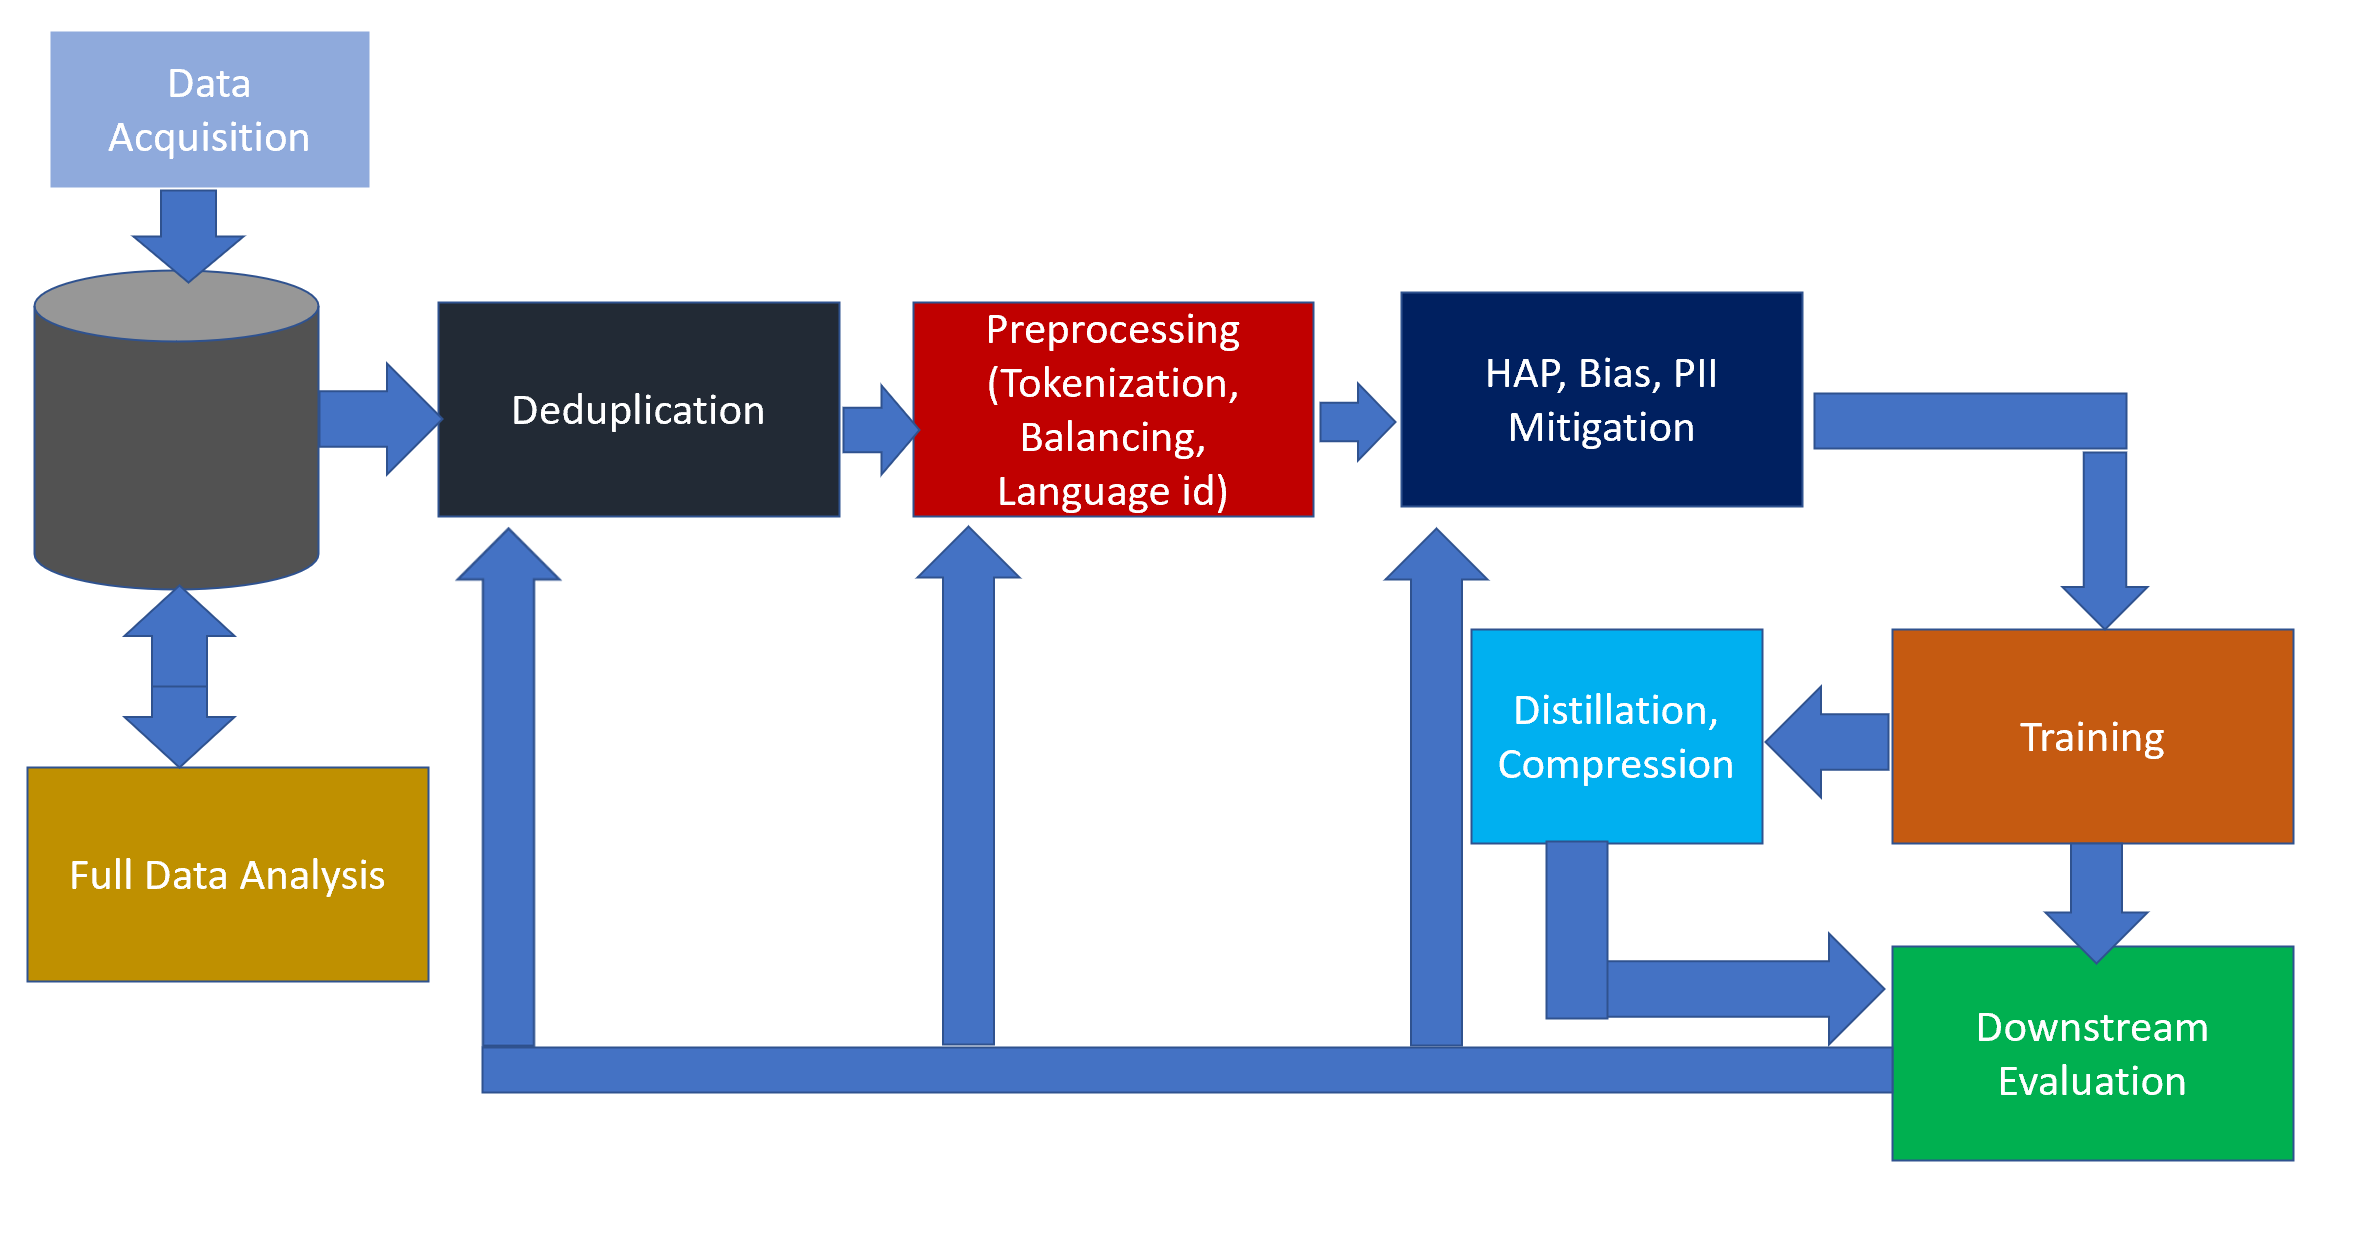
\includegraphics[width = \linewidth]{Figures/sustain3.png}
             \caption{A typical preprocessing pipeline}
             \label{fig:model-preprocess}
         \end{figure}

        The datasets are used to train multiple models in various combinations. BERT, for example, was trained using English Wikipedia and BookCorpus. Whereas Multilingual BERT (mBERT) was trained on multilingual Wikipedia over 100+ languages \cite{Jindrich2019}. RoBERTa on English datasets spanning Wikipedia, Stories, OpenWebText, BoockCorpus as well as CC-News. 

        After a model is trained, the model may be distilled to bring it to a form factor which fits certain latency or space budget. For example,  DistilBERT \cite{Sanh2019} and DistilMBERT are based on BERT and mBERT, respectively. After the base model is deployed, if often needs to be continuously trained to maintain accuracy. A model trained before 2019 would not have known about COVID. The frequency of re-training varies. For example, ~\cite{Wu2022} reported re-training in weekly, or daily frequency for two different use cases. 
    }
}
